\documentclass[12pt,a4paper]{report}
\usepackage[utf8]{inputenc}
\usepackage{amsmath}
\usepackage{amsfonts}
\usepackage{amssymb}
\usepackage{amsthm}
\usepackage{hyperref}

\usepackage{multicol}
\usepackage{fancyhdr}
\usepackage[inline]{enumitem}
\usepackage{tikz}
\usepackage{tikz-cd}
\usetikzlibrary{calc}
\usetikzlibrary{shapes.geometric}
\usepackage[margin=0.5in]{geometry}
\usepackage{xcolor}
\usepackage{listings} 

\hypersetup{
    colorlinks=true,
    linkcolor=blue,
    filecolor=magenta,      
    urlcolor=cyan,
    pdftitle={Tensors},
    pdfpagemode=FullScreen,
    }

%\urlstyle{same}

\newcommand{\CLASSNAME}{Math 5301 -- Numerical Analysis}
\newcommand{\STUDENTNAME}{Paul Carmody}
\newcommand{\ASSIGNMENT}{Homework \#4 }
\newcommand{\DUEDATE}{March 26, 2025}
\newcommand{\SEMESTER}{Spring 2025}
\newcommand{\SCHEDULE}{MW 2:00 to 3:15}
\newcommand{\ROOM}{Crawford 330}

\newcommand{\MMN}{M_{m\times n}}
\newcommand{\FF}{\mathcal{F}}

\pagestyle{fancy}
 	\fancyhf{}
\chead{ \fancyplain{}{\CLASSNAME} }
%\chead{ \fancyplain{}{\STUDENTNAME} }
\rhead{\thepage}
\newcommand{\LET}{\text{Let }}
%\newcommand{\IF}{\text{if }}
\newcommand{\AND}{\text{ and }}
\newcommand{\OR}{\text{ or }}
\newcommand{\FORSOME}{\text{ for some }}
\newcommand{\FORALL}{\text{ for all }}
\newcommand{\WHERE}{\text{ where }}
\newcommand{\WTS}{\text{ WTS }}
\newcommand{\WLOG}{\text{ WLOG }}
\newcommand{\BS}{\backslash}
\newcommand{\DEFINE}[1]{\textbf{\emph{#1}}}
\newcommand{\IF}{$(\Rightarrow)$}
\newcommand{\ONLYIF}{$(\Leftarrow)$}
\newcommand{\ITH}{\textsuperscript{th} }
\newcommand{\FST}{\textsuperscript{st} }
\newcommand{\SND}{\textsuperscript{nd} }
\newcommand{\TRD}{\textsuperscript{rd} }
\newcommand{\INV}{\textsuperscript{-1} }

\newcommand{\XXX}{\mathfrak{X}}
\newcommand{\MMM}{\mathfrak{M}}
%\newcommand{\????}{\textfrak{A}}
%\newcommand{\????}{\textgoth{A}}
%\newcommand{\????}{\textswab{A}}

\DeclareMathOperator{\DER}{Der}
\DeclareMathOperator{\SGN}{sgn}

%%%%%%%
% derivatives
%%%%%%%

\newcommand{\PART}[2]{\frac{\partial #1}{\partial #2}}
\newcommand{\SPART}[2]{\frac{\partial^2 #1}{\partial #2^2}}
\newcommand{\DERIV}[2]{\frac{d #1}{d #2}}
\newcommand{\LAPLACIAN}[1]{\frac{\partial^2 #1}{\partial x^2} + \frac{\partial^2 #1}{\partial y^2}}

%%%%%%%
% sum, product, union, intersections
%%%%%%%

\newcommand{\SUM}[2]{\underset{#1}{\overset{#2}{\sum}}}
\newcommand{\PROD}[2]{\underset{#1}{\overset{#2}{\prod}}}
\newcommand{\UNION}[2]{\underset{#1}{\overset{#2}{\bigcup}}}
\newcommand{\INTERSECT}[2]{\underset{#1}{\overset{#2}{\bigcap}}}
\newcommand{\FSUM}{\SUM{n=-\infty}{\infty}}
       

%%%%%%%
% supremum and infimum
%%%%%%%

\newcommand{\SUP}[1]{\underset{#1}\sup \,}
\newcommand{\INF}[1]{\underset{#1}\inf \,}
\newcommand{\MAX}[1]{\underset{#1}\max \,}
\newcommand{\MIN}[1]{\underset{#1}\min \,}

%%%%%%%
% infinite sums, limits
%%%%%%%

\newcommand{\SUMK}{\SUM{k=1}{\infty}}
\newcommand{\SUMN}{\SUM{n=1}{\infty}}
\newcommand{\SUMKZ}{\SUM{k=0}{\infty}}
\newcommand{\LIM}[1]{\underset{#1}\lim\,}
\newcommand{\IWOB}[1]{\LIM{#1 \to \infty}}
\newcommand{\LIMK}{\IWOB{k}}
\newcommand{\LIMN}{\IWOB{n}}
\newcommand{\LIMX}{\IWOB{x}}
\newcommand{\NIWOB}{\LIM{n \to \infty}}
\newcommand{\LIMSUPK}{\underset{k\to\infty}\limsup \,}
\newcommand{\LIMSUPN}{\underset{n\to\infty}\limsup \,}
\newcommand{\LIMINFK}{\underset{k\to\infty}\liminf \,}
\newcommand{\LIMINFN}{\underset{n\to\infty}\liminf \,}
\newcommand{\ROOTRULE}[1]{\LIMSUPK \BARS{#1}^{1/k}}

\newcommand{\CUPK}{\bigcup_{k=1}^{\infty}}
\newcommand{\CAPK}{\bigcap_{k=1}^{\infty}}
\newcommand{\CUPN}{\bigcup_{n=1}^{\infty}}
\newcommand{\CAPN}{\bigcap_{n=1}^{\infty}}

%%%%%%%
% number systems (real, rational, etc.)
%%%%%%%

\newcommand{\REALS}{\mathbb{R}}
\newcommand{\RATIONALS}{\mathbb{Q}}
\newcommand{\IRRATIONALS}{\REALS \backslash \RATIONALS}
\newcommand{\INTEGERS}{\mathbb{Z}}
\newcommand{\NUMBERS}{\mathbb{N}}
\newcommand{\COMPLEX}{\mathbb{C}}
\newcommand{\DISC}{\mathbb{D}}
\newcommand{\HPLANE}{\mathbb{H}}

\newcommand{\R}{\mathbb{R}}
\newcommand{\Q}{\mathbb{Q}}
\newcommand{\Z}{\mathbb{Z}}
\newcommand{\N}{\mathbb{N}}
\newcommand{\C}{\mathbb{C}}
\newcommand{\T}{\mathbb{T}}
\newcommand{\COUNTABLE}{\aleph_0}
\newcommand{\UNCOUNTABLE}{\aleph_1}


%%%%%%%
% Arithmetic/Algebraic operators
%%%%%%%


\DeclareMathOperator{\MOD}{mod}
%\newcommand{\MOD}[1]{\mod #1}
\newcommand{\BAR}[1]{\overline{#1}}
\newcommand{\LCM}{\text{ lcm}}
\newcommand{\ZMOD}[1]{\Z/#1\Z}
\DeclareMathOperator{\VAR}{Var}
%%%%%%%
% complex operators
%%%%%%%

\DeclareMathOperator{\RR}{Re}
%\newcommand{\RE}{\text{Re}}
\DeclareMathOperator{\IM}{Im}
%\newcommand{\IM}{\text{Im}}
\newcommand{\CONJ}[1]{\overline{#1}}
\DeclareMathOperator{\LOG}{Log}
%\newcommand{\LOG}{\text{ Log }}
\newcommand{\RES}[2]{\underset{#1}{\text{res}} #2}

%%%%%%%
% Group operators
%%%%%%%

\newcommand{\AUT}{\text{Aut}\,}
\newcommand{\KER}{\text{ker}\,}
\newcommand{\END}{\text{End}}
\newcommand{\HOM}{\text{Hom}}
\newcommand{\CYCLE}[1]{(\begin{array}{cccccccccc}
		#1
	\end{array})}
\newcommand{\SUBGROUP}{\underset{\text{group}}\subseteq}	
%\newcommand{\SUBGROUP}{\subseteq_g}
\newcommand{\SUBRING}{\underset{\text{ring}}\subseteq}
\newcommand{\SUBMOD}{\underset{\text{mod}}\subseteq}
\newcommand{\SUBFIELD}{\underset{\text{field}}\subseteq}
\newcommand{\ISO}{\underset{\text{iso}}\longrightarrow}
\newcommand{\HOMO}{\underset{\text{homo}}\longrightarrow}

%%%%%%%
% grouping (parenthesis, absolute value, square, multi-level brackets).
%%%%%%%

\newcommand{\PAREN}[1]{\left (\, #1 \,\right )}
\newcommand{\BRACKET}[1]{\left \{\, #1 \,\right \}}
\newcommand{\SQBRACKET}[1]{\left [\, #1 \,\right ]}
\newcommand{\ABRACKET}[1]{\left \langle\, #1 \,\right \rangle}
\newcommand{\BARS}[1]{\left |\, #1 \,\right |}
\newcommand{\DBARS}[1]{\left \| \, #1 \,\right \|}
\newcommand{\LBRACKET}[1]{\left \{ #1 \right .} 
\newcommand{\RBRACKET}[1]{\left . #1 \right \]}
\newcommand{\RBAR}[1]{\left . #1 \, \right |}
\newcommand{\LBAR}[1]{\left | \, #1 \right .}
\newcommand{\BLBRACKET}[2]{\BRACKET{\RBAR{#1}#2}}
\newcommand{\GEN}[1]{\ABRACKET{#1}}
\newcommand{\BINDEF}[2]{\LBRACKET{\begin{array}{ll}
     #1\\
     #2
\end{array}}}

%%%%%%%
% Fourier Analysis
%%%%%%%

\newcommand{\ONEOTWOPI}{\frac{1}{2\pi}}
\newcommand{\FHAT}{\hat{f}(n)}
\newcommand{\FINT}{\int_{-\pi}^\pi}
\newcommand{\FINTWO}{\int_{0}^{2\pi}}
\newcommand{\FSUMN}[1]{\SUM{n=-#1}{#1}}
%\newcommand{\FSUM}{\SUMN{\infty}}
\newcommand{\EIN}[1]{e^{in#1}}
\newcommand{\NEIN}[1]{e^{-in#1}}
\newcommand{\INTALL}{\int_{-\infty}^{\infty}}
\newcommand{\FTINT}[1]{\INTALL #1 e^{2\pi inx\xi} dx}
\newcommand{\GAUSS}{e^{-\pi x^2}}

%%%%%%%
% formatting 
%%%%%%%

\newcommand{\LEFTBOLD}[1]{\noindent\textbf{#1}}
\newcommand{\SEQ}[1]{\{#1\,\}}
\newcommand{\WIP}{\footnote{work in progress}}
\newcommand{\QED}{\hfill\square}
\newcommand{\ts}{\textsuperscript}
\newcommand{\HLINE}{\noindent\rule{7in}{1pt}\\}

%%%%%%%
% Mathematical note taking (definitions, theorems, etc.)
%%%%%%%

\newcommand{\REM}{\noindent\textbf{\\Remark: }}
\newcommand{\DEF}{\noindent\textbf{\\Definition: }}
\newcommand{\THE}{\noindent\textbf{\\Theorem: }}
\newcommand{\COR}{\noindent\textbf{\\Corollary: }}
\newcommand{\LEM}{\noindent\textbf{\\Lemma: }}
\newcommand{\PROP}{\noindent\textbf{\\Proposition: }}
\newcommand{\PROOF}{\noindent\textbf{\\Proof: }}
\newcommand{\EXP}{\noindent\textbf{\\Example: }}
\newcommand{\TRICKS}{\noindent\textbf{\\Tricks: }}


%%%%%%%
% text highlighting
%%%%%%%

\newcommand{\B}[1]{\textbf{#1}}
\newcommand{\CAL}[1]{\mathcal{#1}}
\newcommand{\UL}[1]{\underline{#1}}

%%%%%%
% Linear Algebra
%%%%%%

\newcommand{\COLVECTOR}[1]{\PAREN{\begin{array}{c}
#1
\end{array} }}
\newcommand{\TWOXTWO}[4]{\PAREN{ \begin{array}{c c} #1&#2 \\ #3 & #4 \end{array} }}
\newcommand{\DTWOXTWO}[4]{\BARS{ \begin{array}{c c} #1&#2 \\ #3 & #4 \end{array} }}
\newcommand{\THREEXTHREE}[9]{\PAREN{ \begin{array}{c c c} #1&#2&#3 \\ #4 & #5 & #6 \\ #7 & #8 & #9 \end{array} }}
\newcommand{\DTHREEXTHREE}[9]{\BARS{ \begin{array}{c c c} #1&#2&#3 \\ #4 & #5 & #6 \\ #7 & #8 & #9 \end{array} }}
\newcommand{\NXN}{\PAREN{ \begin{array}{c c c c} 
			a_{11} & a_{12} & \cdots & a_{1n} \\
			a_{21} & a_{22} & \cdots & a_{2n} \\
			\vdots & \vdots & \ddots & a_{1n} \\
			a_{n1} & a_{n2} & \cdots & a_{nn} \\
		\end{array} }}
\newcommand{\SLR}{SL_2(\R)}
\newcommand{\GLR}{GL_2(\R)}
\DeclareMathOperator{\TR}{tr}
\DeclareMathOperator{\BIL}{Bil}
\DeclareMathOperator{\SPAN}{span}

%%%%%%%
%  White space
%%%%%%%

\newcommand{\BOXIT}[1]{\noindent\fbox{\parbox{\textwidth}{#1}}}


\newtheorem{theorem}{Theorem}[section]
\newtheorem{corollary}{Corollary}[theorem]
\newtheorem{lemma}[theorem]{Lemma}

\theoremstyle{definition}
\newtheorem{definition}[theorem]{Definition}
\newtheorem{prop}[theorem]{Proposition}

\theoremstyle{remark}
\newtheorem{remark}[theorem]{Remark}
\newtheorem{example}[theorem]{Example}
%\newtheorem*{proof}[theorem]{Proof}



\newcommand{\RED}[1]{\textcolor{red}{#1}}
\newcommand{\BLUE}[1]{\textcolor{blue}{#1}}
\definecolor{mygreen}{RGB}{28,172,0} % color values Red, Green, Blue
\definecolor{mylilas}{RGB}{170,55,241}

\begin{document}
\lstset{language=Matlab,%
    %basicstyle=\color{red},
    breaklines=true,%
    morekeywords={matlab2tikz},
    keywordstyle=\color{blue},%
    morekeywords=[2]{1}, keywordstyle=[2]{\color{black}},
    identifierstyle=\color{black},%
    stringstyle=\color{mylilas},
    commentstyle=\color{mygreen},%
    showstringspaces=false,%without this there will be a symbol in the places where there is a space
    numbers=left,%
    numberstyle={\tiny \color{black}},% size of the numbers
    numbersep=9pt, % this defines how far the numbers are from the text
    emph=[1]{for,end,break},emphstyle=[1]\color{red}, %some words to emphasise
    %emph=[2]{word1,word2}, emphstyle=[2]{style},    
}

\begin{center}
	\Large{\CLASSNAME -- \SEMESTER} \\
	\large{ w/Professor Du}
\end{center}
\begin{center}
	\STUDENTNAME \\
	\ASSIGNMENT -- \DUEDATE\\
\end{center} 
\HLINE

\textbf{Assignment:} Consider 1D Poisson Equation $-\Delta x = \sin (\pi x)$, over the region $(0, \pi/2)$ with boundary conditions $u(0)=0$ and $u(\pi/2)=1$.  Using central difference scheme and a mesh of 128, obtain a linear system of $Au = f$ for the problem, then the solve the system using the following methods until a relative residual of $10^{-4}$ is reached. For all methods below, plot the analytical solution, the numerical solution and the error distribution.  Use zero vectors as your initial guess.

\begin{enumerate}[label=(\alph*)]
\item Jacobis's Method.  Plot the rate of convergence and compareit with analysis.
\item Steepest Descent Method. Compare the rate of convergence with that obtained in (a).

\end{enumerate}
\HLINE
%
%
%In the report, please include basic introduction of the methods, all related computer code and plots, as well as all the necessary analysis
%
%
\begin{center}
	\Large{Analytical and Numerical Solutions to Poisson's Equation}
\end{center}

\noindent\textbf{Introduction:}\\

	We will begin by describing the equation and providing an analytical solution.  Then solve this equation using Jacobi's Method and the Steepest Descent Method.  Comparisons will be made as to accurancy and rate of convergence.\\
	
\noindent\textbf{Poison's Equation and an Analytical Solution:}\\

As described in the assignment we will focus our attenion on this Poisson equation and initial conditions.
\begin{align*}
	-\Delta x &= \sin(\pi x)\\
	u(0) = 0 &\AND u(\pi/2)=1.
\end{align*}When we solve this problem analtyically we get
\begin{align*}
	u'(x) &= \int -\sin(\pi x) dx \\
	&= \frac{1}{\pi}\cos(\pi x)+C \\
	u(x) &= \int \PAREN{\frac{1}{\pi}\cos(\pi x)+C} dx \\
	&= \frac{1}{\pi^2}sin(\pi x) + Cx + D \\
	u(0) = 0 &= \frac{1}{\pi^2}sin(\pi 0) + Cx + D \\
	D &= 0 \\
	u(\pi/2) =1 &= \frac{1}{\pi^2}sin(\pi^2/2) + C(\pi/2) \\
	C &= \frac{2\PAREN{1-\frac{1}{\pi^2}}sin(\pi^2/2)}{\pi^2}=\frac{2\PAREN{1-\frac{1}{9.869604064}}0.086022097}{9.869604064} = 1.998233797 \approx 2 \\
%	u(\pi/2) =1 &= \frac{1}{\pi^2}sin(\pi/2) + C(\pi/2) \\
%	C &= \frac{2}{\pi}\PAREN{1-\frac{1}{\pi^2}}\\
%	u(x) &= \frac{1}{\pi^2}sin(\pi x) + \frac{2}{\pi}\PAREN{1-\frac{1}{\pi^2}}x \\
	u(x) &\approx \frac{1}{\pi^2}sin(\pi x) + 2x \\
%	\frac{2\PAREN{1-\frac{1}{\pi^2}}sin(\pi^2/2)}{\pi^2} &= \frac{2\PAREN{1-\frac{1}{9.869604064}}0.086022097}{9.869604064} = 1.998233797 \approx 2
\end{align*}

\noindent\textbf{Centered Difference Scheme}\\

We will attempt to approximate the curve of  the solution at particular points $u_i$ by calculating a slope at a point by using the preceeding point $u_{i-1}$ and succeeding point $u_{i+1}$.  
\begin{align*}
	\frac{u_{i+1}-2u_i+u_{i-1}}{h^2} \approx -\sin (\pi x)
\end{align*}where $h=(\pi/2)/129=\pi/258$ (we use $N+1$ as we start with the left boundary 0).  This can be reduced to 
\begin{align*}
	-u_{i+1}+2u_i-u_{i-1} = h^2\sin (\pi x).
\end{align*}This expands to a linear function over the a matrix $A$ and vector $u=\{ u_i \}$ reflecting the left hand side and the value to our function on the right with $f=\{ f_i \}, f_i=\sin(\pi x_i)$ or
\begin{align*}
	Au &= h^2 f\\
	\PAREN{\begin{array}{cccccc}
		2 & -1 & 0 & 0 &\cdots & 0\\
		-1 & 2 & -1 & 0 &\cdots & 0\\
		0 & -1 & 2 & -1 &\cdots & 0\\
		0 & 0 &-1 & 2 & \cdots & 0\\
		\vdots & \vdots & \vdots & \vdots &\ddots & \vdots\\
		0 & 0 & 0 & 0 & \cdots & 2
	\end{array} } \COLVECTOR{ u_1 \\ u_2 \\ u_3 \\ u_4 \\ \vdots \\ u_i } &= h^2 \COLVECTOR{ f_1 \\ f_2 \\ f_3 \\ f_4 \\ \vdots \\ f_i } \\
	u &= h^2 A^{-1} f
\end{align*}remembering the boundary conditions.  Since $A$ is tri-diagonal we can use several methods and compare the cost and efficiency.  The MatLab code for the Central Difference Method is
	\lstinputlisting{ml04.m}

\noindent\textbf{Jacobi's Iteration Method}\\

Since $A$ is a tri-diagonal matrix it can be divided into three separate matrices that add up.  Let $D$ be zero everywhere except the diagonal where it will hold the values of $A_{ii}$ (namely all 2s).  By applying this iteratively we get
\begin{align*}
	u_i^{[k+1]} &= \frac{1}{2}(u_{i-1}^{[k]}+u_{i+1}^{[k]} - h^2 f_i)
\end{align*}Here is the MatLab code used to generate the graphs that follow:
	\lstinputlisting{ml04c_1.m}
	
From this we generate the following graphs.%4452

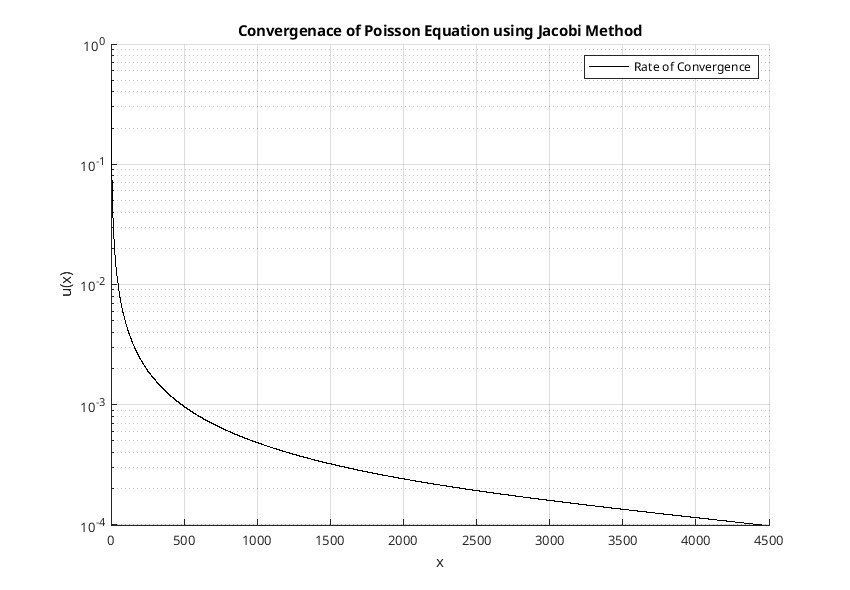
\includegraphics[scale=0.5]{ml04c.png} 

\noindent\textbf{Steepest Descent Method}\\

This technique for approximating our solution to the Poisson equation is to make each iteration in the direction of greatest change.  That is, 
\begin{align*}
	\nabla \phi(u_{k-1}) = Au_{k-1}-f \equiv -r_{k-1}
\end{align*}where $\phi: \R^m \to \R$ of the form
\begin{align*}
	\phi(u) &= \frac{1}{2}u^TAu-u^Tf
\end{align*}which is a quadratic function in $u$ and can be mapped with local extrema either as a top, a bowl or a saddle point, all based on the eigenvalues of $A$ (negative, positive, or neither, respectively).  Thus, when $A$ is SPD we can expect $r_{k}$ to progress ever closer towards the extremum.

This is the source code
	\lstinputlisting{ml04d_1.m}

From this we generate the following graphs.

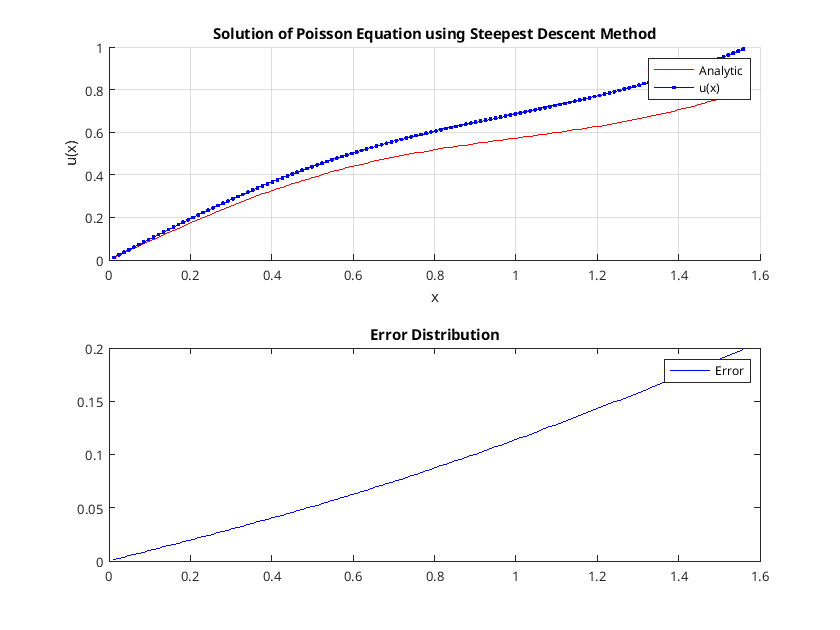
\includegraphics[scale=0.5]{ml04d.png} 

\noindent\textbf{Analyzing the various solutions}.\\

It should be noted that the Jacobi method took 4,452 iterations before being completed and the Steepest Descent Method took 13,454.\\  

The two plots use a logorithmic scale.  A standard scale didn't emphasize the decay rate effectively as the initial iterations showed the great change, so much so that the following improved accuracy couldn't be seen.  The logarithmic scale more effictively shows the improvement.  Each iteration provides very little but necessary improvement.

\end{document}
